\chapter{Resultados y posibles próximos pasos}
\label{chapter:resultados}

Este capítulo está compuesto por dos secciones. En la primera sección se muestran varios resultados y patrones observados durante el análisis explotarorio de los datos de la EFF, y cómo algunos de ellos han influido en la toma de decisiones con respecto a las variables que finalmente han entrado en los modelos. Finalmente, en la segunda sección se comentan los resultados de la evaluación de los diferentes modelos de machine learning utilizados durante este estudio.

Antes de empezar con los resultados, es importante destacar la gran cantidad de variables e información que se recoge en la EFF. En el Cuadro 4.1 se recoge el número de registros y variables disponibles en cada uno de los ficheros utilizados, después de seleccionar sólo a los hogares elegibles para la EFF2020 y a los entrevistadores que participaron en la EFF2017. El número de hogares elegibles para la EFF2020 es de 5.938, el número de entrevistadores en 69 y el número de pantallas que se vieron en el CAPI durante todas las entrevistas es 2.578.926\footnote{Los registros del fichero de paradata son las pantallas del ordenador con las que interactúa el entrevistador durante la entrevista. Suele haber una pregunta por pantalla, y cuando se responde, se pasa a la siguiente pantalla. Cuantas más preguntas, más pantallas se ven.}.

\begin{table}[h]
    \centering{}
    \begin{tabular}{ | l | c | c |}
    \hline
    Nombre del fichero & Registros & Variables \\ \hline
    Fichero de trabajo & 5.938 & 6.103 \\
    Fichero de datos imputados  & 5.938 & 659 \\
    Fichero de recontactos  & 5.938 & 4 \\
    Fichero de contactos  & 5.938 & 636 \\
    Censo de entrevistadores  & 69 & 56 \\
    Fichero paradata  & 2.578.926 & 13 \\
    \hline
    \end{tabular}
    \caption{\textit{Observaciones y variables de los ficheros de la EFF2017}}
\end{table}

Con respecto al número de variables, muchas de ellas en su estado original no son informativas y necesitan ser combinadas con otras para poder obtener información interpretable. Esto reduce considerablemente el número de variables que hay que manejar. Otro grupo importante de variables tienen pocos registros porque se refieren por ejemplo inversiones en activos financieros que sólo tienen unos pocos hogares, y muchas de ellas se descartan, o se adaptan para indicar tenencia de dichos activos. Finalmente, todas las variables que aparecen en el fichero de datos imputados también aparecen en el fichero de trabajo\footnote{El fichero de trabajo es el que recoge todas las correcciones de la revisión y es el que se utiliza para imputar los valores que están missing porque los hogares no los han declarado. Por tanto, la diferencia en las variables que ambos comparten es que en el fichero de datos imputados esas variables están completas porque sus valores missing se han imputado.}. Del fichero de datos imputados se usan las variables con los valores missing imputados, y el fichero de trabajo se utiliza para obtener indicadores de calidad de los datos, indicadores de no-respuesta y otras variables de interés que no aparecen en el fichero de datos imputados.

\section{Análisis exploratorio}

El análisis exploratorio de las variables es fundamental para poder ver cómo son las distribuciones de las variables que se van a utilizar, las relaciones que hay entre ellas, y especialmente la que hay con la variable de interés. También ayuda a detectar posibles errores o particularidades que puedan afectar a los modelos de predicción. Dada la enorme cantidad de variables que se han analizado en este proyecto, en este apartado sólo se presentan algunos resultados que han llamado bastante la atención y se considera que merecen la pena ser nombrados porque ofrecen conocimiento sobre la participación de los panelistas en futuras olas y que podría ser útil en la práctica.

En la figura 4.1 presenta cuatro gráficos de mekko que presentan las propociones de hogares panel que vuelven a participar (región azul) frente a los que no vuelven a hacerlo (región roja) para las variables de número de olas en las que se ha participado (arriba a la izquierda), el nivel de recelo después de la entrevista (arriba a la derecha), el estado de salud reportado por la PR (abajo a la izquerda) y la edad de la PR (abajo a la derecha).

\begin{figure}
	\centering
	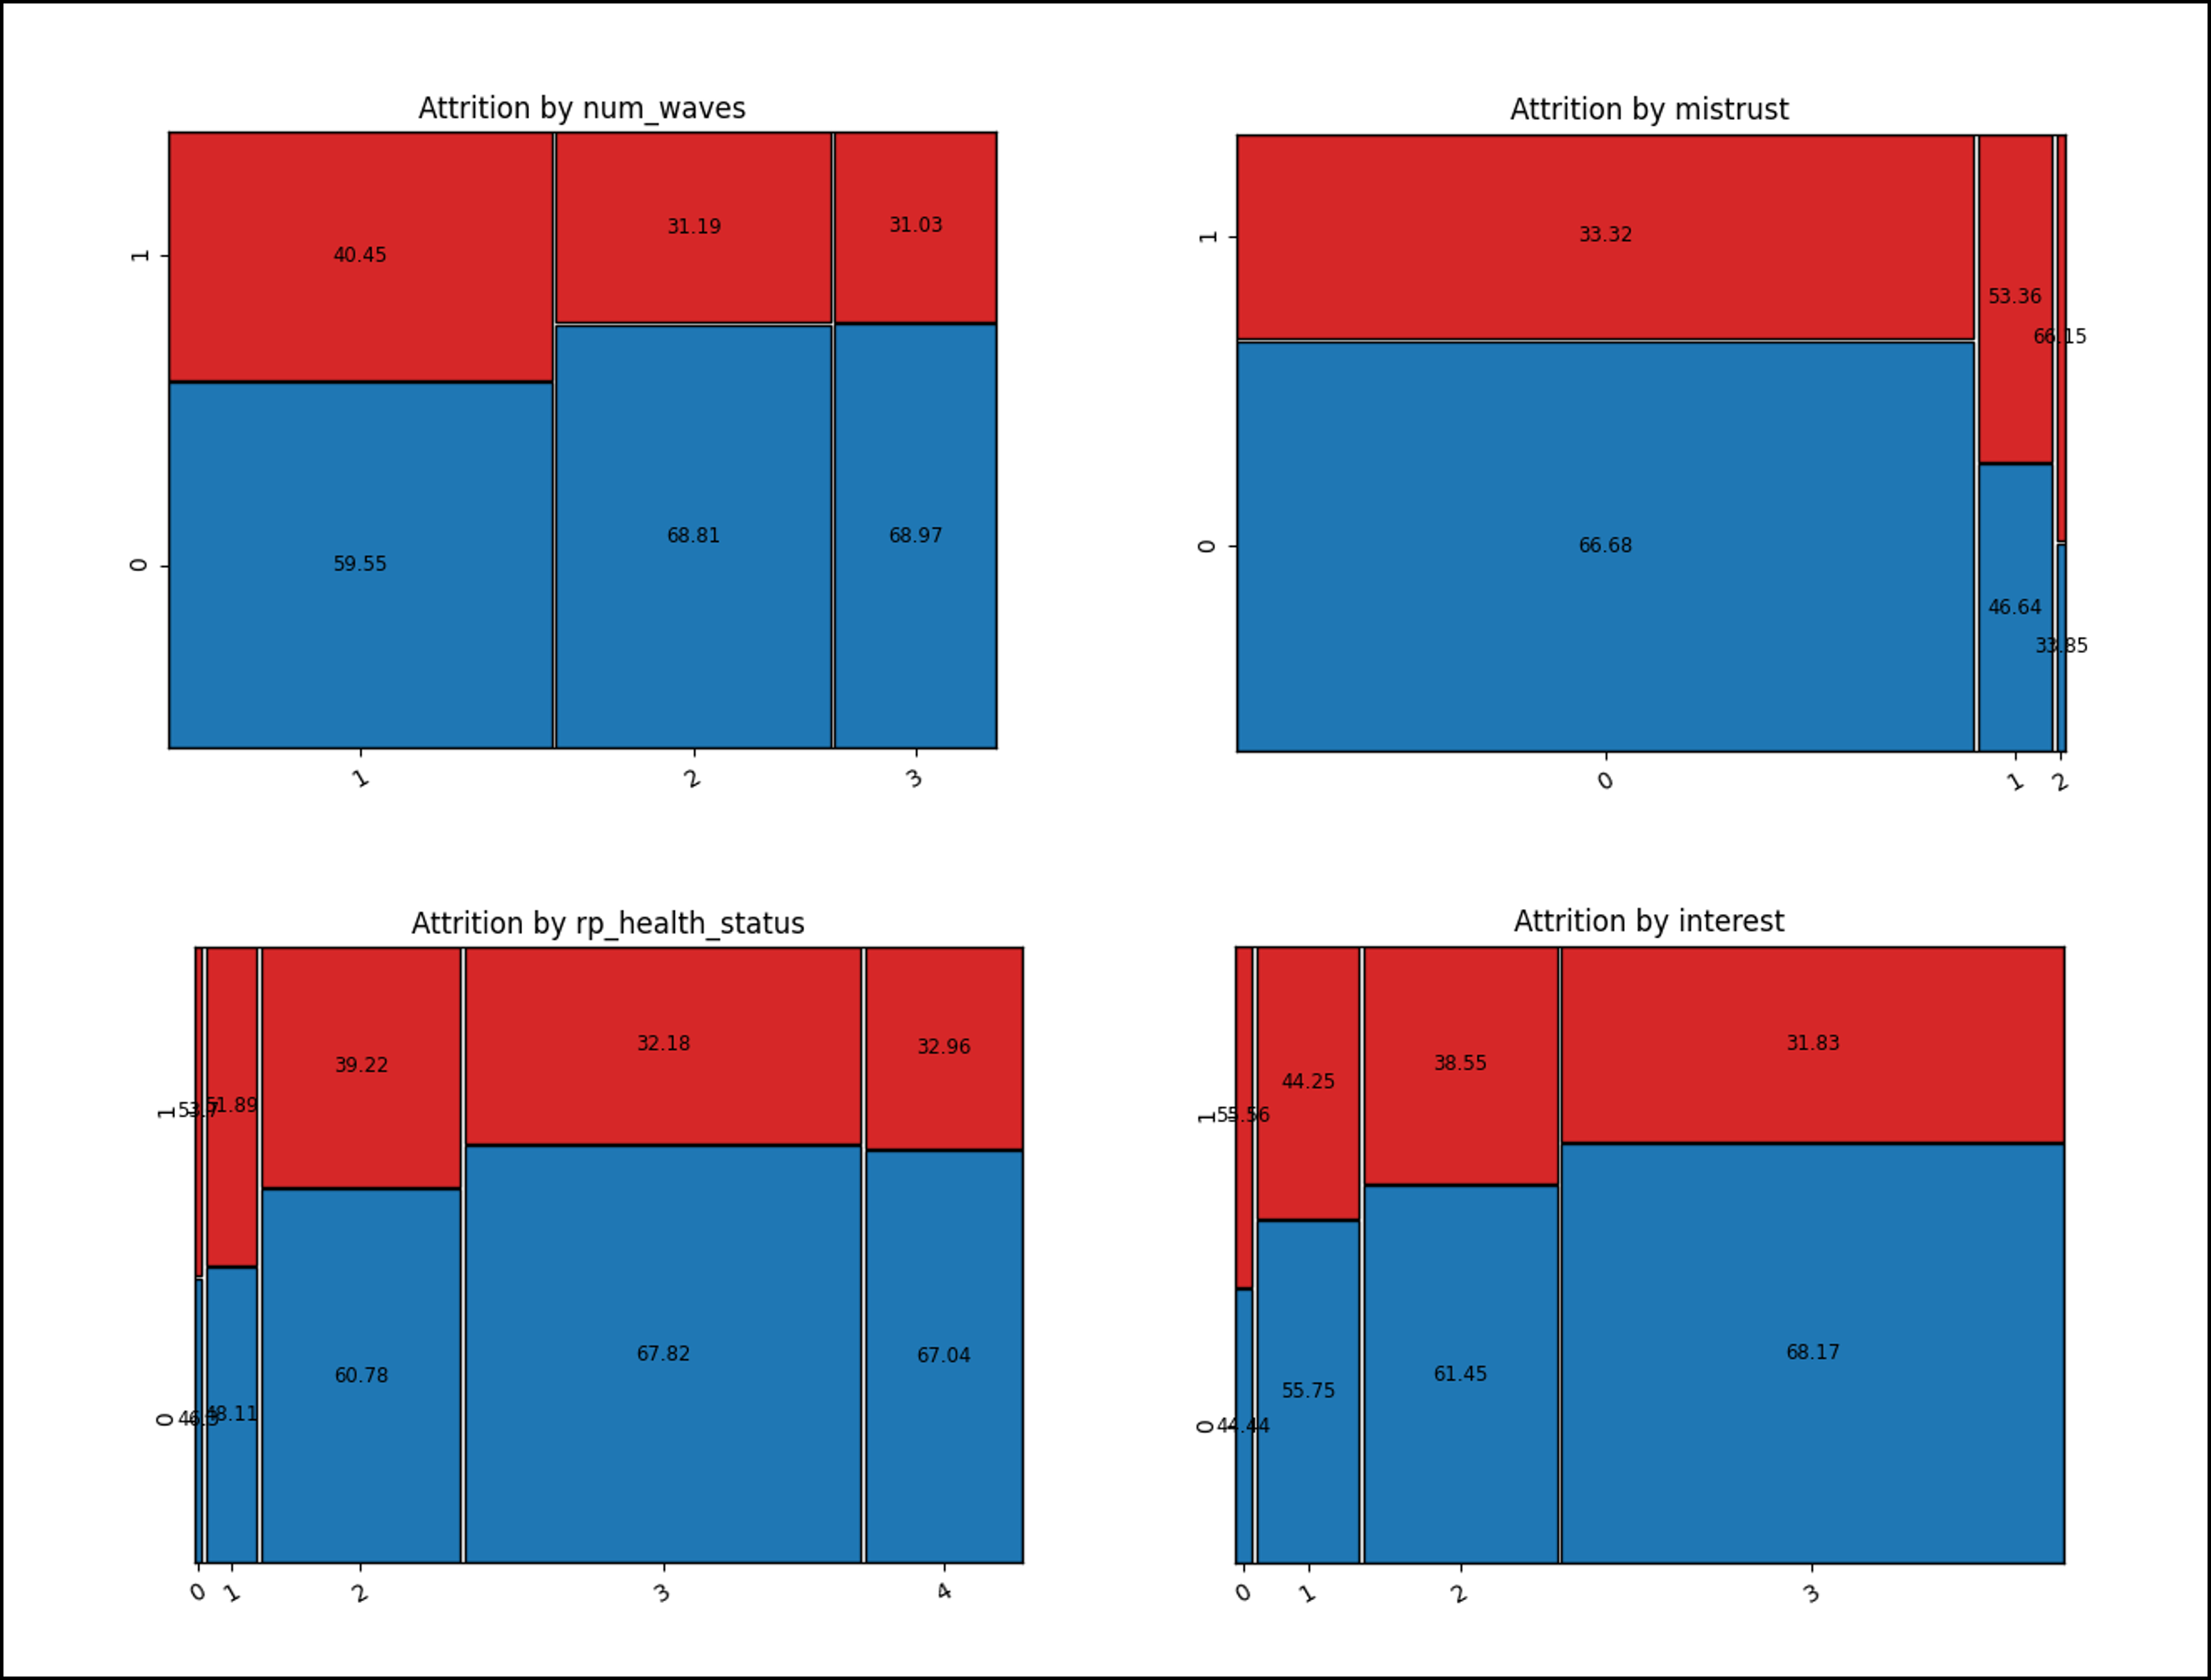
\includegraphics[width=1\textwidth]{figs/categorical.png}
	\caption{Planificación de las actividades del TFM}
	\label{fig:gantt}
\end{figure}

En la figura puede observarse que la proporción de abandono de los hogares que han participado sólo una ola es mayor que la de los que han participado en más de una. Este resultado sugiere que los hogares que llevan menos tiempo en la encuesta podrían ser más complicados de retener, y que podría ser interesante hacer un análisis enfocado en este tipo de hogares.

El segundo resultado a destacar es el del recelo mostrado por el hogar tras la entrevista. Recordemos que en la EFF se hacen preguntan que pueden considerarse delicadas, como por ejemplo si se poseen joyas, o cuál es el saldo que el hogar tiene en su cuenta corriente. Puede ser comprensible que se genere recelo. Este se mide con tres niveles: nada receloso, algo receloso y muy receloso. En el gráfico se observa que la proporción de hogares que abandonan la EFF aumenta con el nivel de recelo. Este resultado es bastante obvio, pero es muy importante resaltarlo porque a un entrevistador podría resultarle muy útil saber si el hogar con el que está a punto de contactar se mostró muy receloso después de hacer la entrevista en la ola anterior, y en su estrategia de contacto y de ganar la cooperación podría hacer más énfasis en los aspectos de la encuesta que causan más recelo.

Finalmente, los dos gráficos de la parte de inferior hacen referencia a características de la PR. En el de la izquierda se observa que la proporción de hogares que abandona la encuesta es mayor cuando menor es el nivel de salud que reporta la PR. De nuevo, esto puede parecer algo obvio porque alguien que tiene peor salud seguramenten o quiera gastar su tiempo en realizar una encuesta. Pero, de nuevo, la estrategia de contacto y de ganar la cooperación de un entrevistador puede adaptarse si ya saben que van a ver a alguien que seguramente tenga mala salud, ya sea ofreciendo hacer la entrevista en varias sesiones, o en un ambiente en el que la PR se muestre más cómoda.

Finalmente, el último gráfico muestra el nivel de interés que mostró la PR durante la entrevista durante la edición anterior. Se observa que la proporción de hogares que vuelven a participar es mayor cuanto mayor es el interés que mostraron durante la ola anterior. De nuevo, se trata de un resultado obvio. Pero, al igual que con el nivel de recelo, este podría ser un dato que podría ser muy útil para el entrevistador cuando esté preparando su estategia de contacto con el hogar.

\section{Evaluación de modelos}

Para la selección de las variables que han entrenado los modelos se han seguido X criterios. En primer lugar, se han seleccionado variables que aparecen en las implementaciones de \cite{kern2021predicting} y \cite{beste2023case} en sus modelos de machine learning. En segundo lugar, se han seleccionado variables sobre factores mencionados en la revisión de \cite{lynn2018tackling} y que han mostrado potencial para predecir la no participación de hogares panel, como por ejemplo la duración o información sobre los contactos con los hogares. En tercer lugar, se han seleccionado variables específicas que se recogen en la EFF, como la tenencia de activos, deudas o el recelo de los hogares percibido por los entrevistadores. Finalmente, tras seleccionar todas las variables anteriores, se han realizado diversos tests gráficos y estadísticos para detectar variables con correlaciones o dependencias muy altas, y se han descartado. La selección final de variables es la que aparece en el cuadro 4.2.

\begin{table}
    \centering
    \begin{tabular}{|l|p{10cm}|}
    \hline
        \textbf{Fuente de información} & \textbf{Variables} \\ \hline
        Características del hogar & Número de adultos que trabajan, Número de adultos jubilados, Propietario vivienda principal, Tamaño del hogar, Tiene otras propiedades, Tiene joyas, Posee negocios, Posee cuentas para pagos, Posee acciones que cotizan, Posee acciones que no cotizan, Posee renta fija, Posee fondos de inversión, Posee cuentas para no pagos, Posee planes de pensiones, Les deben dinero, Poseen vehículos, Percentil de renta, Percentil de riqueza Bruta, Pareja vive en el hogar, Poseen otros activos financieros, Tienen deuda, Tienen ingresos de activos, Hijos viven en el hogar, Nivel de satisfacción con la vida \\ \hline
        Características PR & Nivel de satisfacción con la vida, PR es panel, PR - nivel educativo, PR- Edad, PR - Casada, PR - Viuda, PR - Sexo, Situación laboral - Asalariado, Situación laboral - Jubilado, Situación laboral - Inactivo, PR - Estado de salud \\ \hline
        Valoraciones FI & Recelo tras la entrevista, Tipo de edificio - Unifamiliar, Barreras - portero automático, Barreras - No hay barreras, Entendimiento de las preguntas PR, Interés PR, Razones colaborar - Interesado en estos estudios, Razones para colaborar - Lo lleva el BdE, Razones para colaborar - Relevancia de la encuesta, Razones - Favor al entrevistador, Razones - Dar su opinión, Razones - Otras \\ \hline
        Paradata & PR consiente grabar la entrevista, Hogar con recontacto exitoso, Número de olas en las que se ha participado, Tamaño del municipio, Entrevista con proxy, Número de miembros del hogar que participan, Ratio estricto, Ratio amplio, Número de variables con valores missing, Duración de la entrevista \\ \hline
    \end{tabular}
    \caption{Selección de variables para entrenar los modelos de predicción}
\end{table}

El cuadro 4.3 contiene los resultados del rendimiento de los modelos entrenados sobre el conjunto de test, es decir, los resultados para predecir la no participación de los panelistas en la EFF2022. Las métricas de evaluación que se utilizan son Accuracy, Precision, Recall, F1 y ROC AUC. La métrica de referencia que utilizamos para la evaluación es la ROC AUC, que se encuentra en la parte derecha del cuadro. Esta métrica mide el rendimiento entre la tasa de falsos positivos y falsos negativos. Toma valores de 0.5 a 1, con 1 siendo un predictor perfecto, y 0.5 el que se obtendría con una estimación realizada de manera aleatoria.

\begin{table}[ht]
    \centering
    \begin{tabular}{lccccc}
    \hline
        \textbf{Modelo} & \textbf{Accuracy} & \textbf{Precision} & \textbf{Recall} & \textbf{F1} & \textbf{ROC AUC} \\ \hline
        Logit & 0,6556 & 0,3749 & 0,3573 & 0,3659 & 0,5959 \\ 
        CART & 0,6434 & 0,3338 & 0,2835 & 0,3066 & 0,5521 \\ 
        Random Forest & 0,6489 & 0,3529 & 0,3148 & 0,3328 & 0,5821 \\ 
        XGBooster & 0,6718 & 0,3772 & 0,2769 & 0,3194 & 0,5911 \\ 
        Naive Bayes & 0,6254 & 0,3504 & 0,4063 & 0,3763 & 0,5798 \\ \hline
    \end{tabular}
    \caption{Métricas de evaluación de los modelos de predicción en el conjunto de test}
\end{table}


El modelo de referencia de este estudio, el Logit, presenta una ROC AUC de 0,5959. Se considera que un valor inferior a 0,6 es un resultado malo, por lo que el modelo Logit no es un buen predictor. Con respecto a los otros modelos, observamos que el CART y el Naïve Bayes presentan valores más bajos que el Logit, de 0,5521 y 0,5798 respectivamente. El Random Forest y el XGBooster, en cambio, presentan valores de 0,5821 y 0,5911 respectivalente, que son ligeramente superiores al del modelo Logit.

De estos resultados podemos ver que los modelos de Random Forest y XGBooster mejoran al Logit de referencia. Y entre estos dos, el Random Forest presenta valores un poco más altos en Accuracy y en Precision, y el XGBooster es mejor en Recall y F1. Aun así, es necesario recalcar que el valor de ROC AUC sigue estando por debajo de 0,6, por lo que, aunque se mejore el rendimiento con respecto al modelo Logit, los resultados de los test son malos.

Estos resiltados indican que hay modelos de machine learning que mejoran en rendimiento de la predicción con respecto a un Logit. Sin embargo, las métricas señalan que el rendimiento del mejor modelo es regular. La pregunta que hay que preguntarse entonces es, ¿por qué no está funcionando bien la predicción?

Una de las causas puede ser el overfitting, es decir, que los modelos no son capaces de generalizar bien porque se han adaptado demasiado bien a los datos con los que han sido entrenados, y por tanto su rendimiento no es bueno cuando se les presenta con datos nuevos. una manera de comprobar esto es haciendo el ejercicio predicción sobre los datos de entrenamiento con estos mismos modelos, y ver cómo son esos resultados. Estos resultados pueden verse en el cuadro 4.4.

\begin{table}[ht]
    \centering
    \begin{tabular}{lccccc}
    \hline
        \textbf{Modelo} & \textbf{Accuracy} & \textbf{Precision} & \textbf{Recall} & \textbf{F1} & \textbf{ROC AUC} \\ \hline
        Logit & 0,6389 & 0,4905 & 0,4518 & 0,4704 & 0,6517 \\ 
        CART & 0,6126 & 0,4594 & 0,5178 & 0,4868 & 0,6188 \\ 
        Random Forest & 0,6596 & 0,5223 & 0,4770 & 0,4986 & 0,6726 \\ 
        XGBooster & 0,6544 & 0,5144 & 0,4675 & 0,4898 & 0,6722 \\ 
        Naive Bayes & 0,6251 & 0,4741 & 0,5178 & 0,4950 & 0,6435 \\ \hline
    \end{tabular}
    \caption{Métricas de evaluación de los modelos de predicción en el conjunto de entrenamiento}
\end{table}

Como era de esperar, los resultados de las predicciones de los modelos sobre los datos de entrenamiento son mejores que los que se observan con respecto a los datos test. En este caso, el modelo que presenta mejor rendimiento es el Random Forest, con una métrica de ROC AUC de 0,6726, ligeramente superior a la del XGBooster. El resto de métricas del Ranfom Forest también son ligeramente mejores que las del XGBooster. Sin embargo, esta métrica de ROC AUC está entre 0,6 y 0,75, que lo clasifica como un test regular.

Continuando con el Random Forest, una ventaja de los modelos basados en árboles con respecto a otros modelos es que pueden ser interpretados. En el caso del Radom Forest, es posible consultar qué variables han tenido más peso a la hora de clasificar la participación de los hogares. Aunque los resultados de la predicción del training no sean buenos, merece la pena echarle un ojo por los patrones que haya podido detectar. El cuadro 4.5 presenta las 10 variables con más importancia en el modelo de Random Forest.

\begin{table}[ht]
    \centering
    \begin{tabular}{lc}
    \hline
        \textbf{Variable} & \textbf{Importancia} \\ \hline
        PR es panel & 0,0822 \\ 
        Interés PR & 0,0790 \\ 
        Razones para colaborar - Relevancia de la encuesta & 0,0605 \\ 
        Ratio amplio & 0,0594 \\ 
        Poseen vehículos & 0,0539 \\ 
        Tienen deuda & 0,0496 \\ 
        Situación laboral - Asalariado & 0,0475 \\ 
        Razones colaborar - Interesado en estos estudios & 0,0380 \\ 
        Posee planes de pensiones & 0,0353 \\ 
        PR consiente grabar la entrevista & 0,0348 \\ \hline
    \end{tabular}
    \caption{Selección de variables para entrenar los modelos de predicción}
\end{table}

La importancia de una variable en el Random Forest mide el peso relativo que ha tenido una variable concreta a la hora de crear las ramificaciones de los diferentes árboles de decisiones que va generando el Random Forest durante su entrenamiento. En este caso de la participación en la EFF2020, las tres variables que más importancia tuvieron fueron que la PR fuera panel, que la PR mostrase interés durante la entrevista, y que el entrevitador indicase que el hogar colaboró por la relevancia de la encuesta. También es interesante destacar la variable ratio amplio, que es un indicador de la no-respuesta del hogar a la hora de facilitar cantidades monerarias\footnote{El ratio amplio se define como el cociente entre el número de preguntas en euros respondidas por el hogar, ya fuera como valor puntual o como intervalos, sobre el número total de preguntas planteadas. Cuando mayor es su valor, más información ha facilitado el hogar.}. Finalmente, otra variable que es importante para hacer la clasificación es si la PR consintió que se grabase la entrevista.